\chapter{Trassierungsaufgaben}

\section{Definition}

\begin{flushleft}
    Das Ziel von Trassierungsaufgaben ist es anhand von bestimmten Angaben eine Funktion aufzustellen.
    Deshalb ist das Verstehen der Aufgabenstellung der schwierigste Teil der Aufgabe.
\end{flushleft}

\section{Beispiel}

\begin{flushleft}
    Das ist eine mögliche Aufgabenstellung: \\
    \textit{Eine quadratische Funktion hat im Punkt $P(0|0)$ eine Nullstelle und im Punkt $Q(2|5)$ ein Maximum. Stelle die Funktionsgleichung auf!} \\
    \begin{enumerate}
        \item {
                Die ersten drei Wörter des Satzes: \textbf{\textit{Eine quadratische Funktion}} sagen uns um welchen Typ Funktion es sich handelt.
                Es ist eine quadratische Funktion. Die allgemeine quadratische Funktion sieht so aus:
                \begin{align}
                    f(x)=ax^2+bx+c
                \end{align}
                Unsere Funktion $f$ hat also drei unbekannte, $a$, $b$ und $c$.
            }
        \item {
                Außerdem ist für uns wichtig, dass die Funktion \textbf{\textit{im Punkt $P(0|0)$ eine Nullstelle}} hat.
                Das bedeutet, dass $f(0)=0$ sein muss.
                Unsere erste Bedingung ist also:
                \begin{align}
                    f(0)=0
                \end{align}
            }
        \item {
                Als letztes hat unsere Funktion \textbf{\textit{im Punkt $Q(2|5)$ ein Maximum}}. \\
                Um die Extrempunkte von einer Funktion (hier: $g$) zu finden, muss man die erste Ableitung dieser Funktion gleich $0$ setzen.
                \begin{align}
                    g'(x)=0
                \end{align}
                Im Idealfall bekommt man eine oder mehr Lösungen heraus, wir nennen die Lösung $x_1$.
                Um herauszufinden um welche Art von Extrempunkt es sich handelt setzen wir $x_1$ in die zweite Ableitung von $g$ ein.
                \begin{align}            
                    g''(x) =
                    \begin{cases}
                        \text{Maximum}, &\text{wenn } x < 0 \\
                        \text{Minimum}, &\text{wenn } x > 0
                    \end{cases}
                \end{align}
                Jetzt können wir drei weitere Bedingungen für unsere Aufgabe aufstellen.
                Unsere Funktion soll ein Maximum in $Q(2|5)$ haben, deshalb müssen diese Bedingungen erfüllt sein:
                \begin{align}
                    f(2)=5 \\
                    f'(2)=0 \\
                    f''(2) < 0
                \end{align}
            }
        \item {
                Jetzt müssen wir aus unseren vier Bedingungen eine Funktion bilden, dafür bilden wir erstmal die ersten beiden Ableitungen.
                \begin{align}
                    f(x)&=ax^2+bx+c \\
                    f'(x)&=2ax+b \\
                    f''(x)&=2a \\
                    f(0)&=0 \\
                    f(2)&=5 \\
                    f'(2)&=0 \\
                    f''(2) & < 0
                \end{align}
                Nun müssen wir einsetzen, Ungleichungen ($f''(2) < 0$) dürfen nicht eingesetzt werden.
                \begin{align}
                    0^2a+0b+c &=0 \\
                    c &=0 \\
                    a*2^2+2b+c &= 5 \\
                    4a+2b+c &= 5 \\
                    4a+2b &= 5 \\
                    2a*2+b &=0 \\
                    4a+b &= 0
                \end{align}
                Eine von den drei unbekannten ist gelöst ($c=0$).
                Jetzt muss $4a+2b=5$ in $4a+b=0$ eingesetzt werden.
                \begin{align}
                    4a+2b &=5 \\
                    4a+b &= 0 \\
                    4a+2b-(4a+b) &= 5 \\
                    b &= 5 \\
                    4a+5 &= 0 \\
                    a &= \frac{-5}{4}
                \end{align}
                Alle unbekannten Variablen sind gelöst, $a=\frac{-5}{4}$, $b=5$, $c=0$.
                Also ist das unsere Funktion:
                \begin{align}
                    f(x)=\frac{-5}{4}x^2+5x
                \end{align}
            }
    \end{enumerate}
\end{flushleft}

\begin{center}
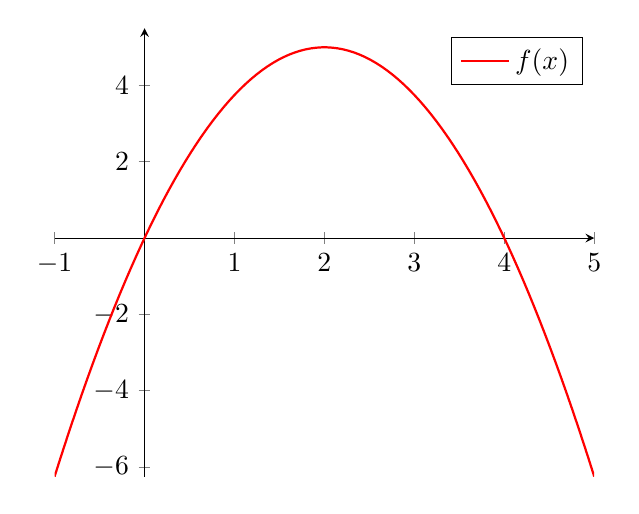
\begin{tikzpicture}   
\begin{axis}[
    axis lines=middle,
    samples=100,
    domain=-1:5,
    ymax=5.5,
    every axis plot/.append style={thick},
]
\addplot[
    color=red,
]
{(-5/4)*((\x)*(\x))+(5)*(\x)};
\addlegendentry{$f(x)$}

\end{axis}
\end{tikzpicture}
\end{center}
